\newpage

\section{Реализация системы}

\subsection{Докеризация}

\subsubsection*{Для чего нужен Docker}

Чтобы использовать MySQL нам нужно устанавливать LAMP (Linux, Apache, MySQL, PHP).
Это будет не удобно, если нужно будет разварачивать на нескольких компьютерах,
так как ручной ввод команд будет занимать много времени.
Чтобы автоматизировать ввод команд в курсовом проекте использовался Docker и docker-compose.

Вместо Docker и docker-compose можно было использовать решения, такие как Denwer и OpenServer,
но для этого нам нужно иметь эти программы на каждом компьютере. Имея один файл docker-compose
в проекте убивает проблему установки больших дистрибутивов, таких как OpenServer.

\subsubsection*{Включаем WSL в Windows 10}

Для работы Docker на Windows 10 нам нужен WSL2 (Windows subsystem for Linux version 2).

Заходим в <<Control Panel>>, затем <<Programs>>, затем <<Turn Windows features on or off>>.

В окне <<Windows Features>> выбираем галочкой следующие пункты:

\begin{itemize}
    \item Hyper-V
    \item Virtual Machine Platform
    \item Windows Hypervisor Platform
    \item Windows Subsystem for Linux
\end{itemize}

Скриншот <<Windows Features>> на
\textbf{рис.~\ref{fig:gpi_pz_controlPanelSettings}~(стр.~\pageref{fig:gpi_pz_controlPanelSettings})}.

\begin{figure}[!hp]
    \centering
    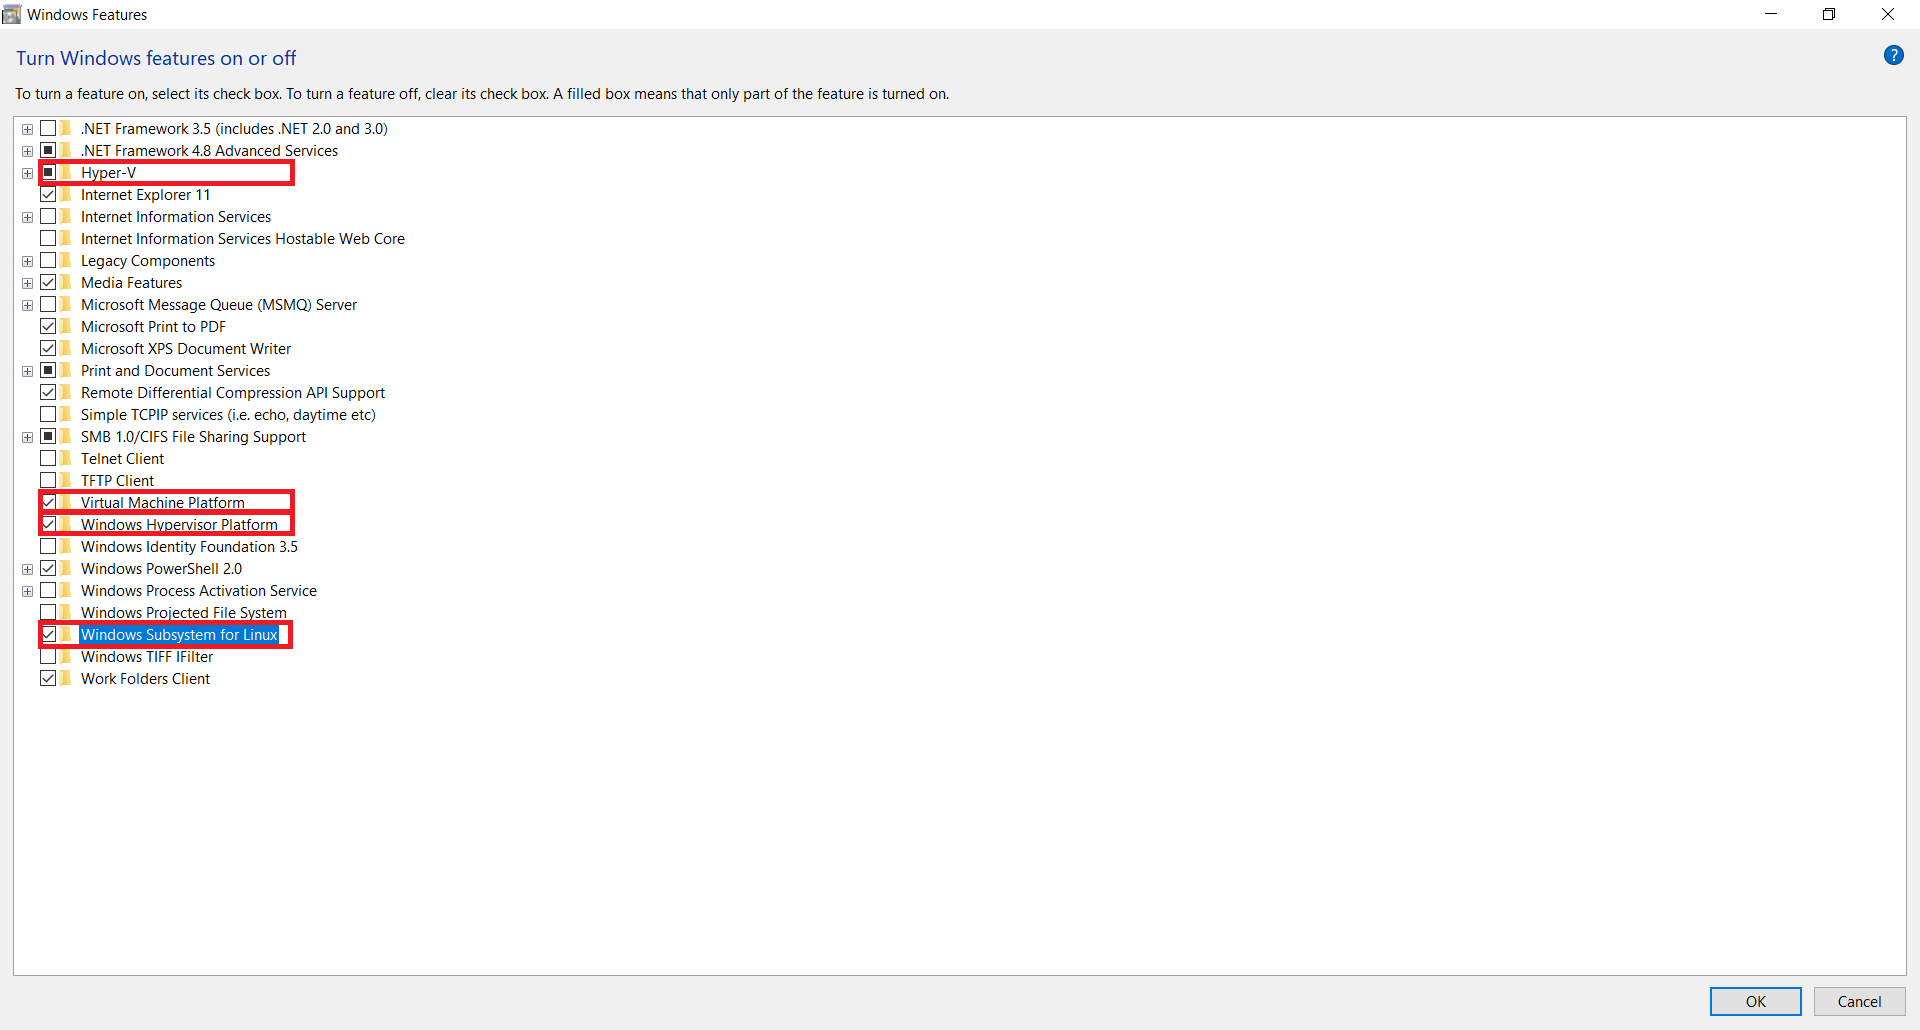
\includegraphics[width=16cm]
        {_assets/gpi_pz_controlPanelSettings.png}
    \caption{Включаем пункты в Панели управления}
    \label{fig:gpi_pz_controlPanelSettings}
\end{figure}

Перезагружаем компьютер - и теперь у нас есть WSL, но только версии 1.

\subsubsection*{Ubuntu в Windows 10}

После того как мы включили функцию WSL мы не имеет никакой операционной системы.
Ubuntu можно скачать из приложения <<Microsoft Store>> по поиску.
Скриншот <<Microsoft Store>> на
\textbf{рис.~\ref{fig:gpi_pz_storeUbuntu}~(стр.~\pageref{fig:gpi_pz_storeUbuntu})}.

\begin{figure}[!hp]
    \centering
    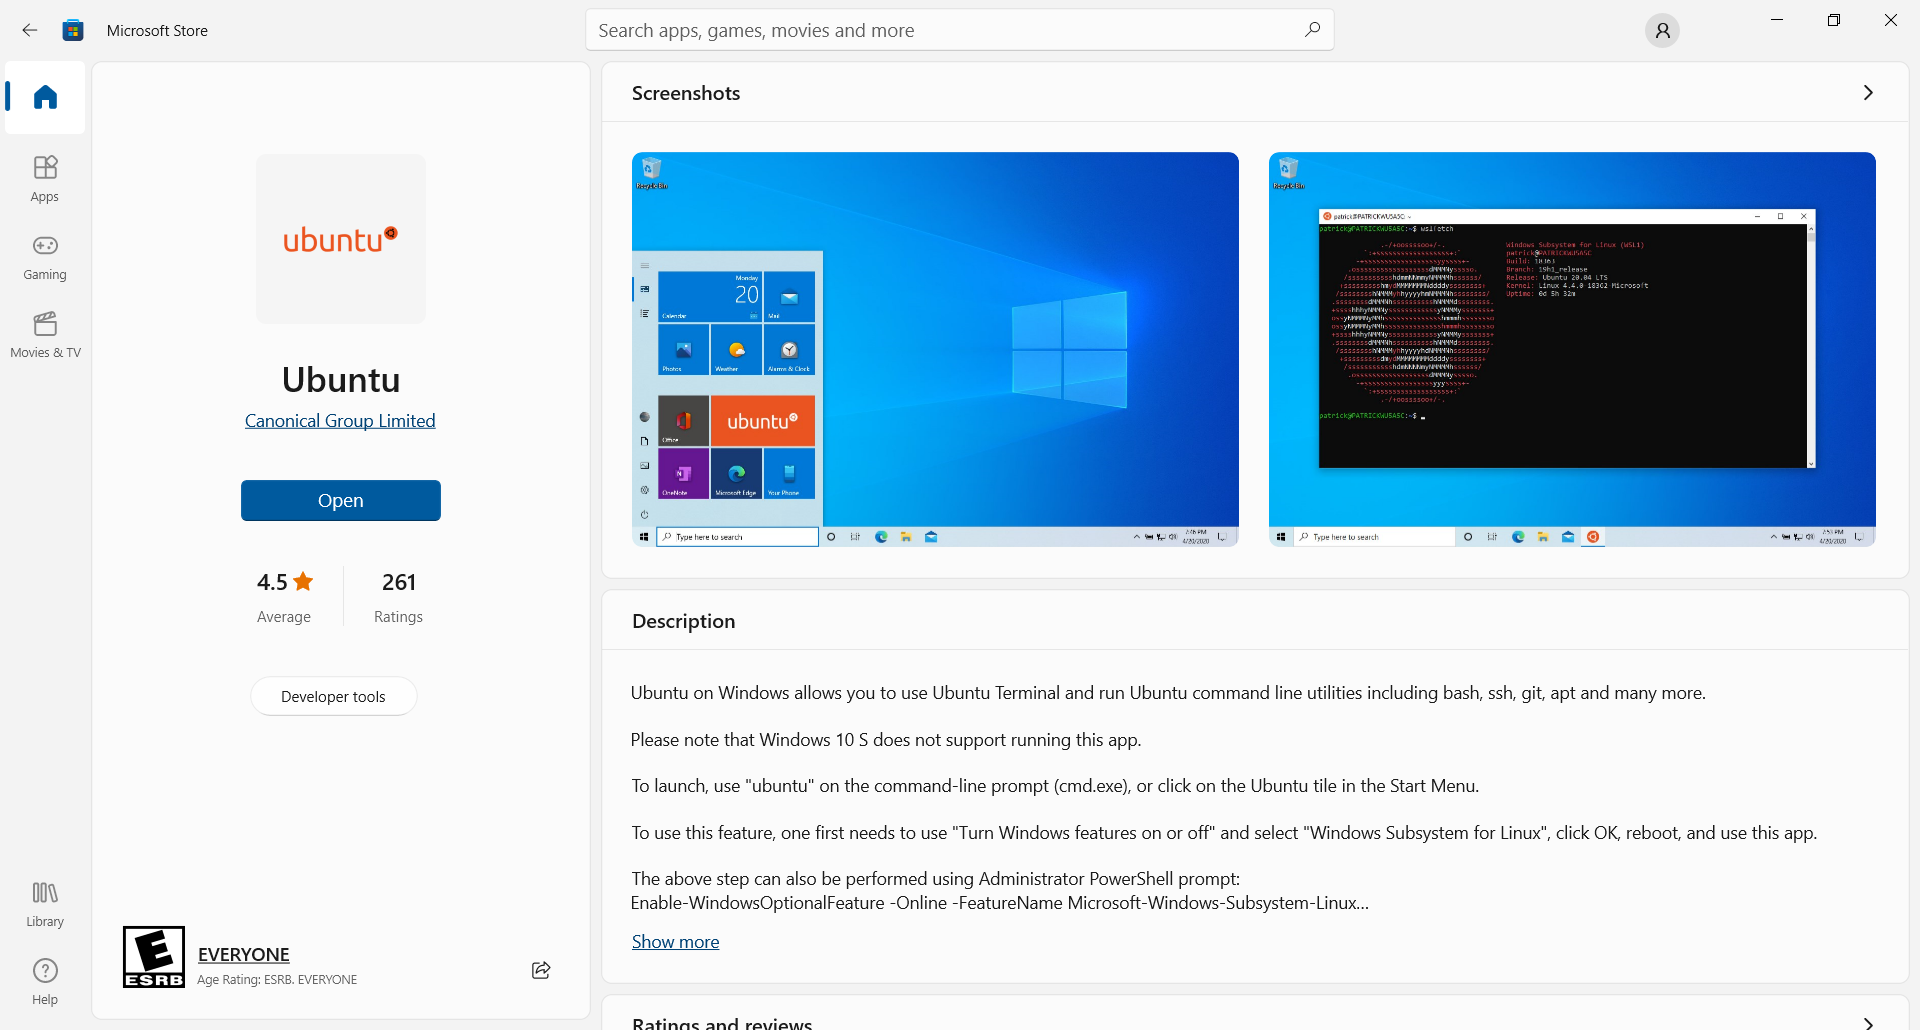
\includegraphics[width=16cm]
        {_assets/gpi_pz_storeUbuntu.png}
    \caption{Скачиваем Ubuntu из Microsoft Store}
    \label{fig:gpi_pz_storeUbuntu}
\end{figure}

\newpage

\subsection{Скрипты для запуска проектов}

В ходе написания курсовой работы были разработаны следующие проекты:

\begin{itemize}
    \item Backend для API на Express.
    \item Frontend для панели администратора на React.
    \item Frontend для интернет-магазина на React.
    \item LAMP для MySQL.
\end{itemize}

Для того чтобы запускать каждый проект нужено входить в каждую папку (папку проекта)
и запускать свой скрипт. Было принято решение записать все команды в один файл - Makefile,
который находится в корне репозитория.

\lstinputlisting[
    name=\textbf{Листинг: Makefile},
    language=make,
    numbers=none,
]
    {../Makefile}

\newpage
